\documentclass[]{article}
\usepackage{lmodern}
\usepackage{amssymb,amsmath}
\usepackage{ifxetex,ifluatex}
\usepackage{fixltx2e} % provides \textsubscript
\ifnum 0\ifxetex 1\fi\ifluatex 1\fi=0 % if pdftex
  \usepackage[T1]{fontenc}
  \usepackage[utf8]{inputenc}
\else % if luatex or xelatex
  \ifxetex
    \usepackage{mathspec}
  \else
    \usepackage{fontspec}
  \fi
  \defaultfontfeatures{Ligatures=TeX,Scale=MatchLowercase}
\fi
% use upquote if available, for straight quotes in verbatim environments
\IfFileExists{upquote.sty}{\usepackage{upquote}}{}
% use microtype if available
\IfFileExists{microtype.sty}{%
\usepackage{microtype}
\UseMicrotypeSet[protrusion]{basicmath} % disable protrusion for tt fonts
}{}
\usepackage[margin=1in]{geometry}
\usepackage{hyperref}
\hypersetup{unicode=true,
            pdftitle={Suffolk 2019},
            pdfborder={0 0 0},
            breaklinks=true}
\urlstyle{same}  % don't use monospace font for urls
\usepackage{color}
\usepackage{fancyvrb}
\newcommand{\VerbBar}{|}
\newcommand{\VERB}{\Verb[commandchars=\\\{\}]}
\DefineVerbatimEnvironment{Highlighting}{Verbatim}{commandchars=\\\{\}}
% Add ',fontsize=\small' for more characters per line
\usepackage{framed}
\definecolor{shadecolor}{RGB}{248,248,248}
\newenvironment{Shaded}{\begin{snugshade}}{\end{snugshade}}
\newcommand{\AlertTok}[1]{\textcolor[rgb]{0.94,0.16,0.16}{#1}}
\newcommand{\AnnotationTok}[1]{\textcolor[rgb]{0.56,0.35,0.01}{\textbf{\textit{#1}}}}
\newcommand{\AttributeTok}[1]{\textcolor[rgb]{0.77,0.63,0.00}{#1}}
\newcommand{\BaseNTok}[1]{\textcolor[rgb]{0.00,0.00,0.81}{#1}}
\newcommand{\BuiltInTok}[1]{#1}
\newcommand{\CharTok}[1]{\textcolor[rgb]{0.31,0.60,0.02}{#1}}
\newcommand{\CommentTok}[1]{\textcolor[rgb]{0.56,0.35,0.01}{\textit{#1}}}
\newcommand{\CommentVarTok}[1]{\textcolor[rgb]{0.56,0.35,0.01}{\textbf{\textit{#1}}}}
\newcommand{\ConstantTok}[1]{\textcolor[rgb]{0.00,0.00,0.00}{#1}}
\newcommand{\ControlFlowTok}[1]{\textcolor[rgb]{0.13,0.29,0.53}{\textbf{#1}}}
\newcommand{\DataTypeTok}[1]{\textcolor[rgb]{0.13,0.29,0.53}{#1}}
\newcommand{\DecValTok}[1]{\textcolor[rgb]{0.00,0.00,0.81}{#1}}
\newcommand{\DocumentationTok}[1]{\textcolor[rgb]{0.56,0.35,0.01}{\textbf{\textit{#1}}}}
\newcommand{\ErrorTok}[1]{\textcolor[rgb]{0.64,0.00,0.00}{\textbf{#1}}}
\newcommand{\ExtensionTok}[1]{#1}
\newcommand{\FloatTok}[1]{\textcolor[rgb]{0.00,0.00,0.81}{#1}}
\newcommand{\FunctionTok}[1]{\textcolor[rgb]{0.00,0.00,0.00}{#1}}
\newcommand{\ImportTok}[1]{#1}
\newcommand{\InformationTok}[1]{\textcolor[rgb]{0.56,0.35,0.01}{\textbf{\textit{#1}}}}
\newcommand{\KeywordTok}[1]{\textcolor[rgb]{0.13,0.29,0.53}{\textbf{#1}}}
\newcommand{\NormalTok}[1]{#1}
\newcommand{\OperatorTok}[1]{\textcolor[rgb]{0.81,0.36,0.00}{\textbf{#1}}}
\newcommand{\OtherTok}[1]{\textcolor[rgb]{0.56,0.35,0.01}{#1}}
\newcommand{\PreprocessorTok}[1]{\textcolor[rgb]{0.56,0.35,0.01}{\textit{#1}}}
\newcommand{\RegionMarkerTok}[1]{#1}
\newcommand{\SpecialCharTok}[1]{\textcolor[rgb]{0.00,0.00,0.00}{#1}}
\newcommand{\SpecialStringTok}[1]{\textcolor[rgb]{0.31,0.60,0.02}{#1}}
\newcommand{\StringTok}[1]{\textcolor[rgb]{0.31,0.60,0.02}{#1}}
\newcommand{\VariableTok}[1]{\textcolor[rgb]{0.00,0.00,0.00}{#1}}
\newcommand{\VerbatimStringTok}[1]{\textcolor[rgb]{0.31,0.60,0.02}{#1}}
\newcommand{\WarningTok}[1]{\textcolor[rgb]{0.56,0.35,0.01}{\textbf{\textit{#1}}}}
\usepackage{longtable,booktabs}
\usepackage{graphicx,grffile}
\makeatletter
\def\maxwidth{\ifdim\Gin@nat@width>\linewidth\linewidth\else\Gin@nat@width\fi}
\def\maxheight{\ifdim\Gin@nat@height>\textheight\textheight\else\Gin@nat@height\fi}
\makeatother
% Scale images if necessary, so that they will not overflow the page
% margins by default, and it is still possible to overwrite the defaults
% using explicit options in \includegraphics[width, height, ...]{}
\setkeys{Gin}{width=\maxwidth,height=\maxheight,keepaspectratio}
\IfFileExists{parskip.sty}{%
\usepackage{parskip}
}{% else
\setlength{\parindent}{0pt}
\setlength{\parskip}{6pt plus 2pt minus 1pt}
}
\setlength{\emergencystretch}{3em}  % prevent overfull lines
\providecommand{\tightlist}{%
  \setlength{\itemsep}{0pt}\setlength{\parskip}{0pt}}
\setcounter{secnumdepth}{5}
% Redefines (sub)paragraphs to behave more like sections
\ifx\paragraph\undefined\else
\let\oldparagraph\paragraph
\renewcommand{\paragraph}[1]{\oldparagraph{#1}\mbox{}}
\fi
\ifx\subparagraph\undefined\else
\let\oldsubparagraph\subparagraph
\renewcommand{\subparagraph}[1]{\oldsubparagraph{#1}\mbox{}}
\fi

%%% Use protect on footnotes to avoid problems with footnotes in titles
\let\rmarkdownfootnote\footnote%
\def\footnote{\protect\rmarkdownfootnote}

%%% Change title format to be more compact
\usepackage{titling}

% Create subtitle command for use in maketitle
\providecommand{\subtitle}[1]{
  \posttitle{
    \begin{center}\large#1\end{center}
    }
}

\setlength{\droptitle}{-2em}

  \title{Suffolk 2019}
    \pretitle{\vspace{\droptitle}\centering\huge}
  \posttitle{\par}
    \author{}
    \preauthor{}\postauthor{}
    \date{}
    \predate{}\postdate{}
  

\begin{document}
\maketitle

{
\setcounter{tocdepth}{2}
\tableofcontents
}
\hypertarget{about-this-course}{%
\section*{About this course}\label{about-this-course}}
\addcontentsline{toc}{section}{About this course}

This course is an introduction R, RStudio and statistics. Our primary aims are to get comfortable working with R and to be able to prepare, manipulate, analyse and visualise data..

\begin{center}\rule{0.5\linewidth}{\linethickness}\end{center}

Agenda

\hypertarget{introduction-to-r-and-rstudio}{%
\section{Introduction to R and RStudio}\label{introduction-to-r-and-rstudio}}

\hypertarget{learning-objectives}{%
\subsection{Learning objectives}\label{learning-objectives}}

In this session, we will have a look at R and RStudio. We will interact with both and use the various components of RStudio.

\hypertarget{what-is-r}{%
\subsubsection{What is R?}\label{what-is-r}}

R is an environment for statistical computing and graphics. RStudio is an editor or integrated development environment (IDE) that makes working with R much more comfortable.

To install R and RStudio on your computer, download both from the following sources:

\begin{itemize}
\tightlist
\item
  Download R from \href{https://cran.r-project.org}{The Comprehensive R Archive Network (CRAN)}
\item
  Download RStudio from \href{https://www.rstudio.com}{RStudio.com}
\end{itemize}

Keep both R and RStudio up to date. That means go online and check for newer versions. In case there are new versions, download those and re-install.

\hypertarget{rstudio}{%
\subsubsection{RStudio}\label{rstudio}}

Let's get acquainted with R. When you start RStudio for the first time, you'll see three panes:

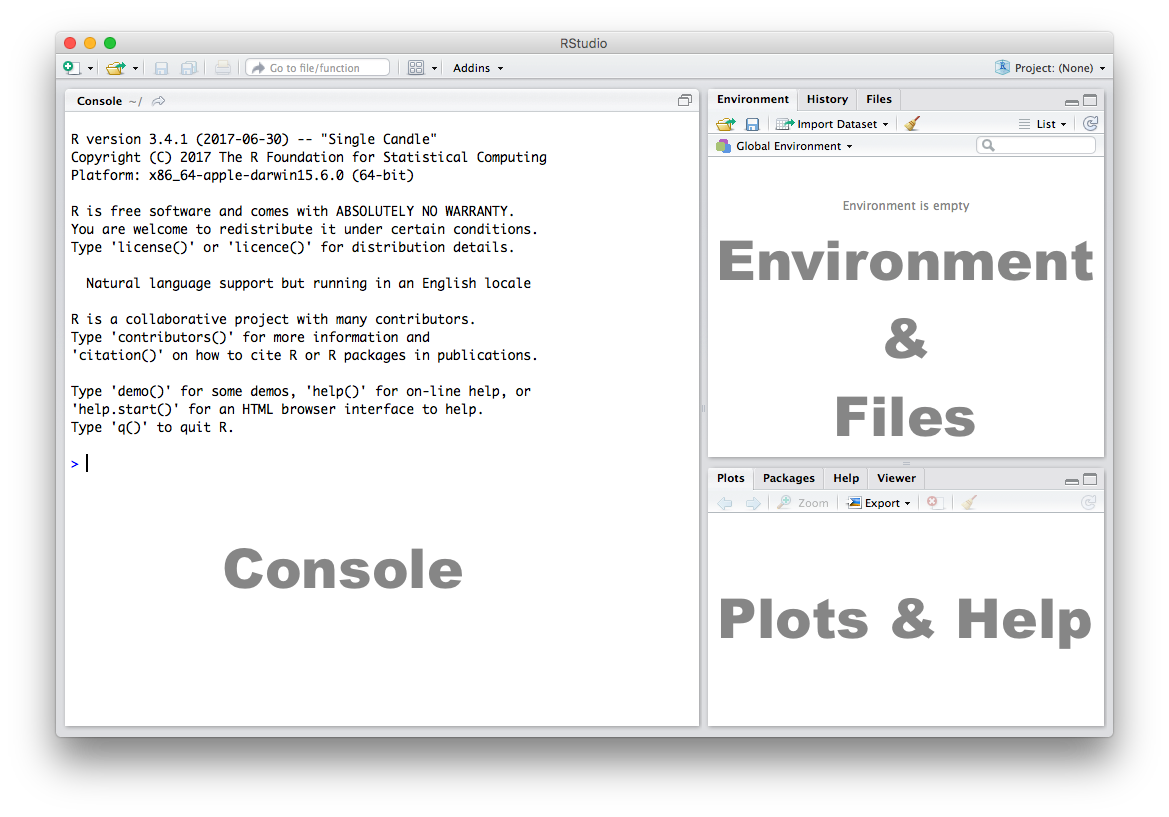
\includegraphics{./img/rstudio_default.png}

\hypertarget{console}{%
\subsubsection{Console}\label{console}}

The Console in RStudio is the simplest way to interact with R. You can type some code at the Console and when you press ENTER, R will run that code. Depending on what you type, you may see some output in the Console or if you make a mistake, you may get a warning or an error message.

Let's familiarize ourselves with the console by using R as a simple calculator:

\begin{Shaded}
\begin{Highlighting}[]
\DecValTok{2} \OperatorTok{+}\StringTok{ }\DecValTok{4}
\end{Highlighting}
\end{Shaded}

\begin{verbatim}
[1] 6
\end{verbatim}

Now that we know how to use the \texttt{+} sign for addition, let's try some other mathematical operations such as subtraction (\texttt{-}), multiplication (\texttt{*}), and division (\texttt{/}).

\begin{Shaded}
\begin{Highlighting}[]
\DecValTok{10} \OperatorTok{-}\StringTok{ }\DecValTok{4}
\end{Highlighting}
\end{Shaded}

\begin{verbatim}
[1] 6
\end{verbatim}

\begin{Shaded}
\begin{Highlighting}[]
\DecValTok{5} \OperatorTok{*}\StringTok{ }\DecValTok{3}
\end{Highlighting}
\end{Shaded}

\begin{verbatim}
[1] 15
\end{verbatim}

\begin{Shaded}
\begin{Highlighting}[]
\DecValTok{7} \OperatorTok{/}\StringTok{ }\DecValTok{2}
\end{Highlighting}
\end{Shaded}

\begin{verbatim}
[1] 3.5
\end{verbatim}

\begin{longtable}[]{@{}ll@{}}
\toprule
\endhead
\begin{minipage}[t]{0.69\columnwidth}\raggedright
You can use the cursor or arrow keys on your keyboard to edit your code at the console:- Use the UP and DOWN keys to re-run something without typing it again- Use the LEFT and RIGHT keys to edit\strut
\end{minipage} & \begin{minipage}[t]{0.25\columnwidth}\raggedright
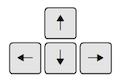
\includegraphics{./img/rstudio_cursorkeys.png}\strut
\end{minipage}\tabularnewline
\bottomrule
\end{longtable}

Take a few minutes to play around at the console and try different things out. Don't worry if you make a mistake, you can't break anything easily!

\hypertarget{scripts}{%
\subsubsection{Scripts}\label{scripts}}

The Console is great for simple tasks but if you're working on a project you would mostly likely want to save your work in some sort of a document or a file. Scripts in R are just plain text files that contain R code. You can edit a script just like you would edit a file in any word processing or note-taking application.

Create a new script using the menu or the toolbar button as shown below.

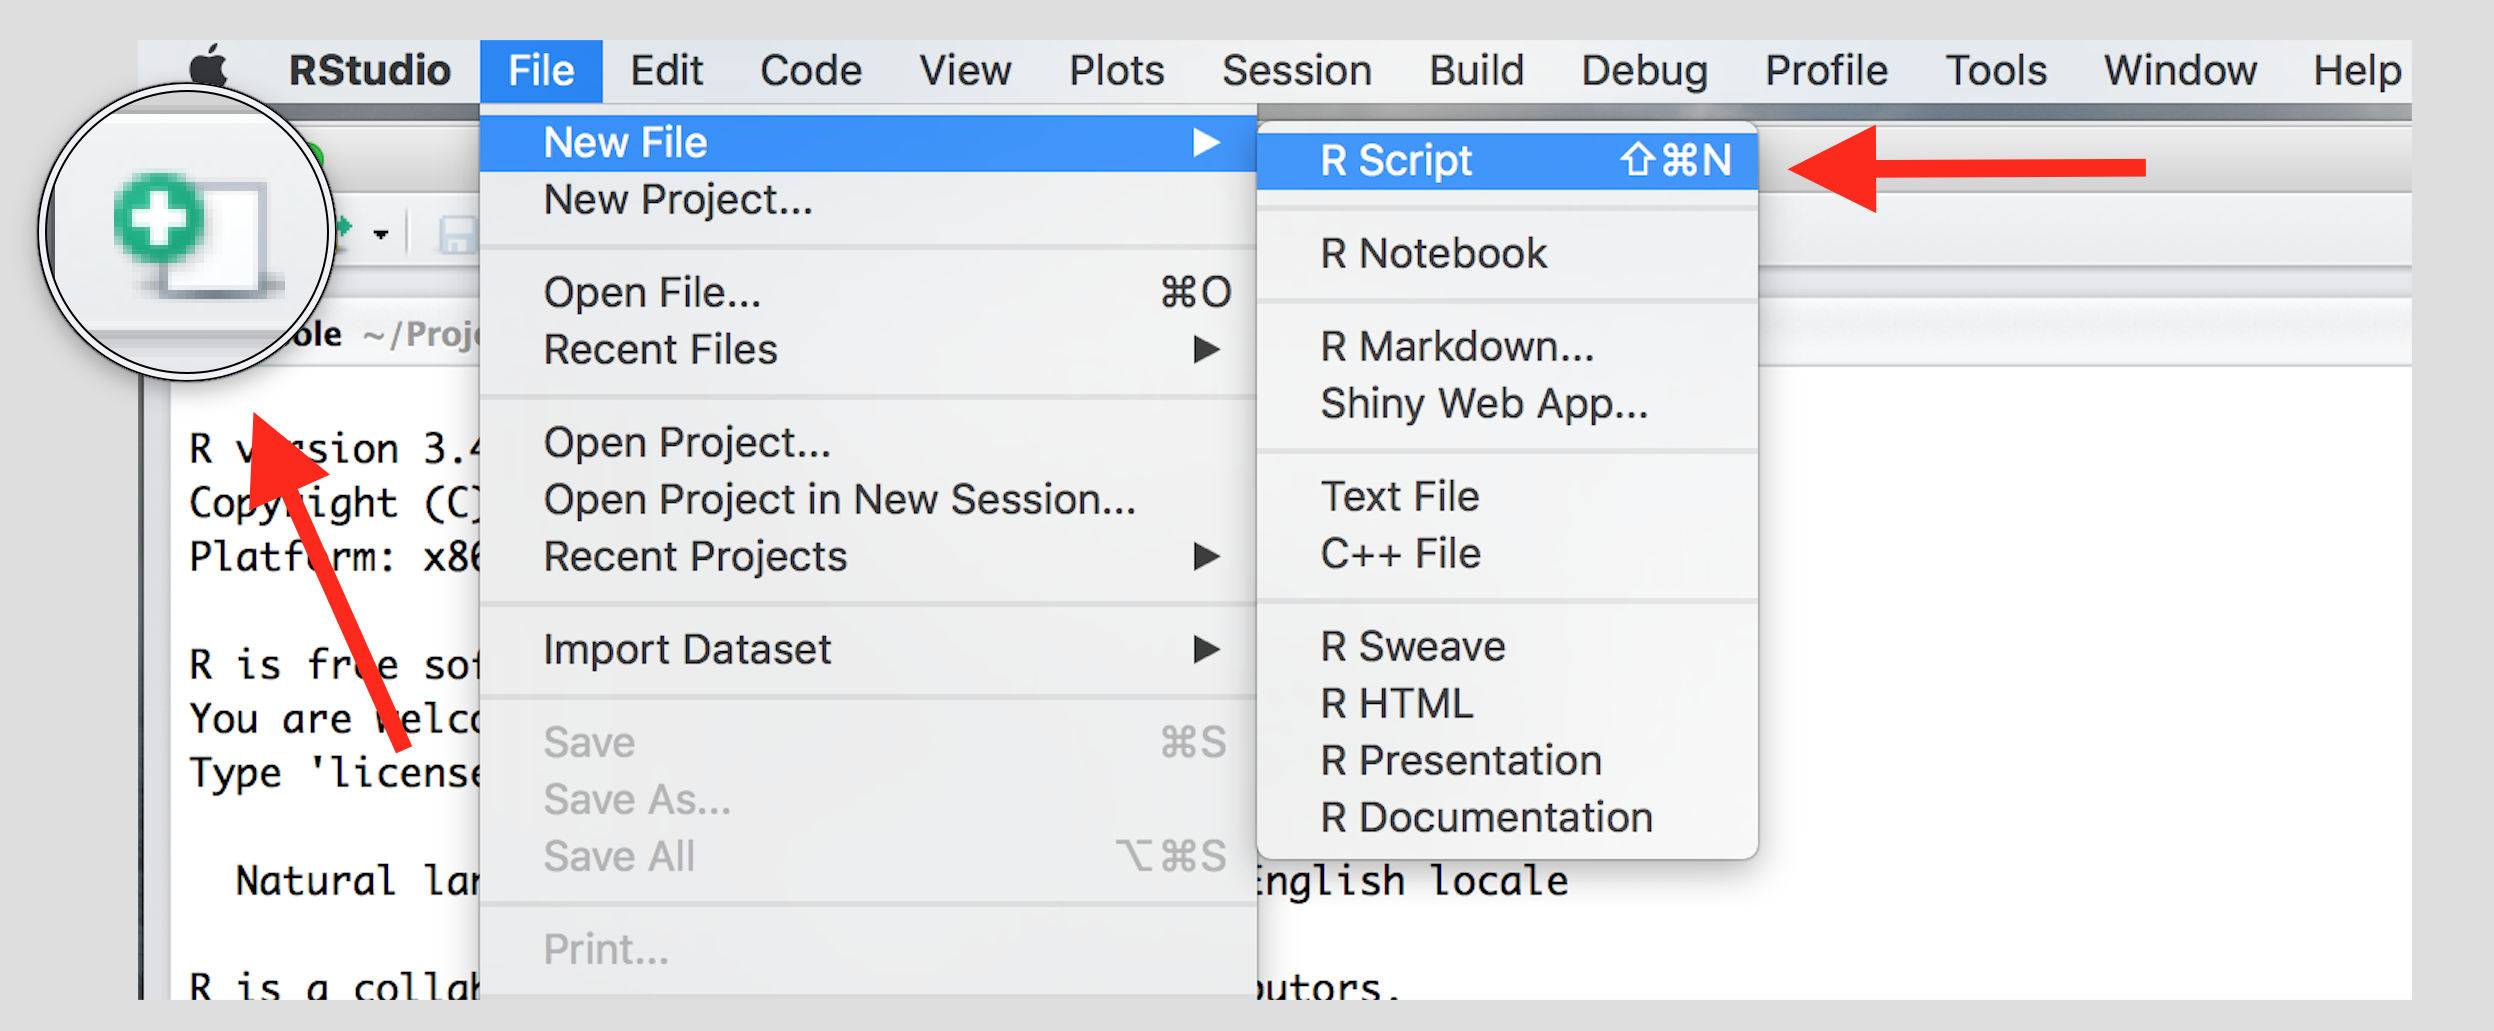
\includegraphics{./img/rstudio_newfile.png}

Once you've created a script, it is generally a good idea to give it a meaningful name and save it immediately. For our first session save your script as \textbf{seminar1.R}

\begin{longtable}[]{@{}ll@{}}
\toprule
\endhead
\begin{minipage}[t]{0.52\columnwidth}\raggedright
Familiarize yourself with the script window in RStudio, and especially the two buttons labeled \textbf{Run} and \textbf{Source}\strut
\end{minipage} & \begin{minipage}[t]{0.42\columnwidth}\raggedright
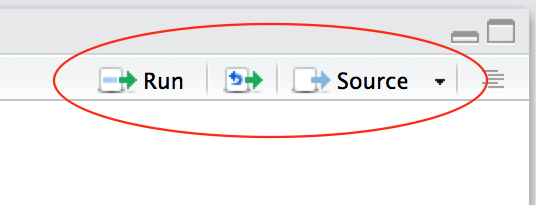
\includegraphics{./img/rstudio_script.png}\strut
\end{minipage}\tabularnewline
\bottomrule
\end{longtable}

There are a few different ways to run your code from a script.

\begin{longtable}[]{@{}ll@{}}
\toprule
\endhead
\begin{minipage}[t]{0.23\columnwidth}\raggedright
One line at a time\strut
\end{minipage} & \begin{minipage}[t]{0.71\columnwidth}\raggedright
Place the cursor on the line you want to run and hit CTRL-ENTER or use the \textbf{Run} button\strut
\end{minipage}\tabularnewline
\begin{minipage}[t]{0.23\columnwidth}\raggedright
Multiple lines\strut
\end{minipage} & \begin{minipage}[t]{0.71\columnwidth}\raggedright
Select the lines you want to run and hit CTRL-ENTER or use the \textbf{Run} button\strut
\end{minipage}\tabularnewline
\begin{minipage}[t]{0.23\columnwidth}\raggedright
Entire script\strut
\end{minipage} & \begin{minipage}[t]{0.71\columnwidth}\raggedright
Use the \textbf{Source} button\strut
\end{minipage}\tabularnewline
\bottomrule
\end{longtable}

\hypertarget{r-syntax-data-structures-and-types}{%
\section{R-syntax, data structures and types}\label{r-syntax-data-structures-and-types}}

\hypertarget{seminar}{%
\subsection{Seminar}\label{seminar}}

In this session we introduce R-syntax, and data types.

\hypertarget{functions}{%
\subsubsection{Functions}\label{functions}}

Functions are a set of instructions that carry out a specific task. Functions often require some input and generate some output. For example, instead of using the \texttt{+} operator for addition, we can use the \texttt{sum} function to add two or more numbers.

\begin{Shaded}
\begin{Highlighting}[]
\KeywordTok{sum}\NormalTok{(}\DecValTok{1}\NormalTok{, }\DecValTok{4}\NormalTok{, }\DecValTok{10}\NormalTok{)}
\end{Highlighting}
\end{Shaded}

\begin{verbatim}
[1] 15
\end{verbatim}

In the example above, \texttt{1,\ 4,\ 10} are the inputs and 15 is the output. A function always requires the use of parenthesis or round brackets \texttt{()}. Inputs to the function are called \textbf{arguments} and go inside the brackets. The output of a function is displayed on the screen but we can also have the option of saving the result of the output. More on this later.

\hypertarget{getting-help}{%
\subsubsection{Getting Help}\label{getting-help}}

Another useful function in R is \texttt{help} which we can use to display online documentation. For example, if we wanted to know how to use the \texttt{sum} function, we could type \texttt{help(sum)} and look at the online documentation.

\begin{Shaded}
\begin{Highlighting}[]
\KeywordTok{help}\NormalTok{(sum)}
\end{Highlighting}
\end{Shaded}

The question mark \texttt{?} can also be used as a shortcut to access online help.

\begin{Shaded}
\begin{Highlighting}[]
\NormalTok{?sum}
\end{Highlighting}
\end{Shaded}

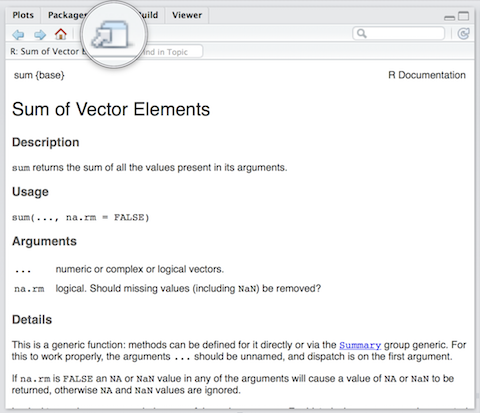
\includegraphics{./img/rstudio_help.png}

Use the toolbar button shown in the picture above to expand and display the help in a new window.

Help pages for functions in R follow a consistent layout generally include these sections:

\begin{longtable}[]{@{}ll@{}}
\toprule
\endhead
Description & A brief description of the function\tabularnewline
Usage & The complete syntax or grammar including all arguments (inputs)\tabularnewline
Arguments & Explanation of each argument\tabularnewline
Details & Any relevant details about the function and its arguments\tabularnewline
Value & The output value of the function\tabularnewline
Examples & Example of how to use the function\tabularnewline
\bottomrule
\end{longtable}

\hypertarget{the-assignment-operator}{%
\subsubsection{The Assignment Operator}\label{the-assignment-operator}}

Now we know how to provide inputs to a function using parenthesis or round brackets \texttt{()}, but what about the output of a function?

We use the assignment operator \textbf{\texttt{\textless{}-}} for creating or updating objects. If we wanted to save the result of adding \texttt{sum(1,\ 4,\ 10)}, we would do the following:

\begin{Shaded}
\begin{Highlighting}[]
\NormalTok{myresult <-}\StringTok{ }\KeywordTok{sum}\NormalTok{(}\DecValTok{1}\NormalTok{, }\DecValTok{4}\NormalTok{, }\DecValTok{10}\NormalTok{)}
\end{Highlighting}
\end{Shaded}

The line above creates a new object called \texttt{myresult} in our environment and saves the result of the \texttt{sum(1,\ 4,\ 10)} in it. To see what's in \texttt{myresult}, just type it at the console:

\begin{Shaded}
\begin{Highlighting}[]
\NormalTok{myresult}
\end{Highlighting}
\end{Shaded}

\begin{verbatim}
[1] 15
\end{verbatim}

Take a look at the \textbf{Environment} pane in RStudio and you'll see \texttt{myresult} there.

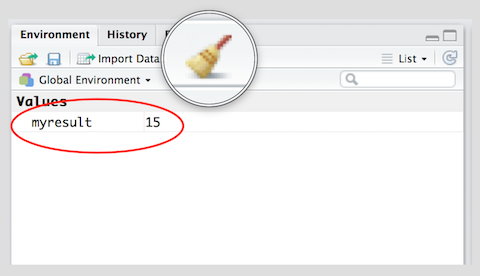
\includegraphics{./img/rstudio_env.png}

To delete all objects from the environment, you can use the \textbf{broom} button as shown in the picture above.

We called our object \texttt{myresult} but we can call it anything as long as we follow a few simple rules. Object names can contain upper or lower case letters (\texttt{A-Z}, \texttt{a-z}), numbers (\texttt{0-9}), underscores (\texttt{\_}) or a dot (\texttt{.}) but all object names must start with a letter. Choose names that are descriptive and easy to type.

\begin{longtable}[]{@{}ll@{}}
\toprule
Good Object Names & Bad Object Names\tabularnewline
\midrule
\endhead
result & a\tabularnewline
myresult & x1\tabularnewline
my.result & this.name.is.just.too.long\tabularnewline
my\_result &\tabularnewline
data1 &\tabularnewline
\bottomrule
\end{longtable}

\hypertarget{sequences}{%
\subsubsection{Sequences}\label{sequences}}

We often need to create sequences when manipulating data. For instance, you might want to perform an operation on the first 10 rows of a dataset so we need a way to select the range we're interested in.

There are two ways to create a sequence. Let's try to create a sequence of numbers from 1 to 10 using the two methods:

\begin{enumerate}
\def\labelenumi{\arabic{enumi}.}
\tightlist
\item
  Using the colon \texttt{:} operator. If you're familiar with spreadsheets then you might've already used \texttt{:} to select cells, for example \texttt{A1:A20}. In R, you can use the \texttt{:} to create a sequence in a similar fashion:
\end{enumerate}

\begin{Shaded}
\begin{Highlighting}[]
\DecValTok{1}\OperatorTok{:}\DecValTok{10}
\end{Highlighting}
\end{Shaded}

\begin{verbatim}
 [1]  1  2  3  4  5  6  7  8  9 10
\end{verbatim}

\begin{enumerate}
\def\labelenumi{\arabic{enumi}.}
\tightlist
\item
  Using the \texttt{seq} function we get the exact same result:
\end{enumerate}

\begin{Shaded}
\begin{Highlighting}[]
\KeywordTok{seq}\NormalTok{(}\DataTypeTok{from =} \DecValTok{1}\NormalTok{, }\DataTypeTok{to =} \DecValTok{10}\NormalTok{)}
\end{Highlighting}
\end{Shaded}

\begin{verbatim}
 [1]  1  2  3  4  5  6  7  8  9 10
\end{verbatim}

The \texttt{seq} function has a number of options which control how the sequence is generated. For example to create a sequence from 0 to 100 in increments of \texttt{5}, we can use the optional \texttt{by} argument. Notice how we wrote \texttt{by\ =\ 5} as the third argument. It is a common practice to specify the name of argument when the argument is optional. The arguments \texttt{from} and \texttt{to} are not optional, se we can write \texttt{seq(0,\ 100,\ by\ =\ 5)} instead of \texttt{seq(from\ =\ 0,\ to\ =\ 100,\ by\ =\ 5)}. Both, are valid ways of achieving the same outcome. You can code whichever way you like. We recommend to write code such that you make it easy for your future self and others to read and understand the code.

\begin{Shaded}
\begin{Highlighting}[]
\KeywordTok{seq}\NormalTok{(}\DataTypeTok{from =} \DecValTok{0}\NormalTok{, }\DataTypeTok{to =} \DecValTok{100}\NormalTok{, }\DataTypeTok{by =} \DecValTok{5}\NormalTok{)}
\end{Highlighting}
\end{Shaded}

\begin{verbatim}
 [1]   0   5  10  15  20  25  30  35  40  45  50  55  60  65  70  75  80
[18]  85  90  95 100
\end{verbatim}

Another common use of the \texttt{seq} function is to create a sequence of a specific length. Here, we create a sequence from 0 to 100 with length 9, i.e., the result is a vector with 9 elements.

\begin{Shaded}
\begin{Highlighting}[]
\KeywordTok{seq}\NormalTok{(}\DataTypeTok{from =} \DecValTok{0}\NormalTok{, }\DataTypeTok{to =} \DecValTok{100}\NormalTok{, }\DataTypeTok{length.out =}  \DecValTok{9}\NormalTok{)}
\end{Highlighting}
\end{Shaded}

\begin{verbatim}
[1]   0.0  12.5  25.0  37.5  50.0  62.5  75.0  87.5 100.0
\end{verbatim}

Now it's your turn:

\begin{itemize}
\tightlist
\item
  Create a sequence of \textbf{odd} numbers between 0 and 100 and save it in an object called \texttt{odd\_numbers}
\end{itemize}

\begin{Shaded}
\begin{Highlighting}[]
\NormalTok{odd_numbers <-}\StringTok{ }\KeywordTok{seq}\NormalTok{(}\DecValTok{1}\NormalTok{, }\DecValTok{100}\NormalTok{, }\DecValTok{2}\NormalTok{)}
\end{Highlighting}
\end{Shaded}

\begin{itemize}
\tightlist
\item
  Next, display \texttt{odd\_numbers} on the console to verify that you did it correctly
\end{itemize}

\begin{Shaded}
\begin{Highlighting}[]
\NormalTok{odd_numbers}
\end{Highlighting}
\end{Shaded}

\begin{verbatim}
 [1]  1  3  5  7  9 11 13 15 17 19 21 23 25 27 29 31 33 35 37 39 41 43 45
[24] 47 49 51 53 55 57 59 61 63 65 67 69 71 73 75 77 79 81 83 85 87 89 91
[47] 93 95 97 99
\end{verbatim}

\begin{itemize}
\item
  What do the numbers in square brackets \texttt{{[}\ {]}} mean? Look at the number of values displayed in each line to find out the answer.
\item
  Use the \texttt{length} function to find out how many values are in the object \texttt{odd\_numbers}.

  \begin{itemize}
  \tightlist
  \item
    HINT: Try \texttt{help(length)} and look at the examples section at the end of the help screen.
  \end{itemize}
\end{itemize}

\begin{Shaded}
\begin{Highlighting}[]
\KeywordTok{length}\NormalTok{(odd_numbers)}
\end{Highlighting}
\end{Shaded}

\begin{verbatim}
[1] 50
\end{verbatim}


\end{document}
